\section{Decision effects and one prospective confirmation}
\label{sec:evidence}
\paragraph{Consumed discovery.}
We use the already consumed E3 IID and new-appearance banks, 2,000 scenes each,
and all five fixed independent/source 64 models. Original image versions, cards,
ties, and stored predictions are retained. The analysis does not recertify any
rule. At fixed restored-model actions, pooled 512 versus direct 512 changes 3.68\%
of labels on IID and 3.83\% on new appearance, all reference-safe to pool-danger
in these observations. Descriptive crossed model/scene 95\% intervals are
[2.89\%,4.53\%] and [3.03\%,4.70\%]. The five models share 2,000 scenes; their
10,000 model--scene entries are not independent trials.

With independent selection by each oracle, pooled 512 loses 72/2,000 IID safe
opportunities (3.60 pp) and 77/2,000 appearance opportunities (3.85 pp). The actual
target 64 oracle loses 60 and 67 respectively. These are full-scene consequences,
not only differences on unselected high-cost candidates. The fixed-footprint
precision check changes .05\% of fixed-action labels on IID and none on appearance.
Pooling flips stable to that check remain 3.63\% and 3.83\%.

Signed cost terms at fixed IID selections are+.001807 from pooling, $-.000653$
from the source raster, and $-.000292$ from the model. On appearance they are
$.002060$, $-.000714$, and $-.001453$, giving total mean $-.000108$ despite mean
absolute error .003102. Model and net measurement terms oppose one another in
31.52\% and 32.49\% of decisions. These are signed cancellations, not causal
percentages attributed by summing absolute components.

\paragraph{Frozen prediction.}
This substantive signal motivates one new normal-IID bank of 2,000 scenes, with
unchanged models, generator, footprints, formulas, threshold, and ties. No new
training is performed. Anonymous continuous patch and full-scene identities have
no exact overlap with the 10,200 E2/E3 records, including training and validation.
This is a same-generator confirmation, not cross-task transfer. The three
predictions require: (H1) stable-reference lost-opportunity probability above .01
for pooled 512; (H2) conservative direction proportion above .90; and (H3) a
small-minus-larger margin flip-rate difference above .10 under joint boundary
overlap. Each claim has one-sided error budget $\gamma=.05/3$.

H1 uses an exact binomial lower bound. H3 uses an approximate crossed model/scene
bootstrap with only five model seeds. An additional stricter H2 scene-level
check was recorded after job submission but before inspecting any new outcome:
among scenes with any selected-action pooling flip across the five fixed models,
all flips in a scene must be conservative. It avoids a degenerate bootstrap lower
limit of one when every observed flip has the same direction. The original
protocol and output remain unchanged; Appendix~\ref{app:direction} gives the
timing and distinguishes the two estimands.

\begin{table}[t]
\centering\small
\caption{Prospective normal-IID confirmation. H1 is the original primary stable
pooled 512 endpoint; the target 64 result is supplementary to the full decomposition.
One-sided lower bounds use $\gamma=.05/3$; H3's bootstrap is approximate.}
\label{tab:confirmation}
\begin{tabular}{p{.39\linewidth}rrr}
\toprule
Prediction & Observation & Lower bound & Criterion\\
\midrule
H1: stable lost opportunities &61/2,000&2.29\%&$>1\%$\\
H2: only conservative changes in a changed scene &68/68&94.16\%&$>90\%$\\
H3: small-minus-larger margin enrichment &37.31 pp&26.06 pp&$>10$ pp\\
\bottomrule
\end{tabular}
\end{table}

\paragraph{What changes in decisions.}
The direct oracle has 1,592 safe opportunities. Pooled 512 accepts 1,529 with no
unsafe outcome observed, losing 63 opportunities (3.15 pp of all scenes). The
finer-property check also retains a safe candidate in 61 of those scenes: H1's
exact lower is 2.2869\%. The actual target 64 oracle accepts 1,540, of which two
are unsafe, so it loses 54/2,000 safe opportunities. This is 2.70 pp of all scenes
and 3.39\% of the 1,592 available opportunities. It is not a 2.7\% increase in
danger, nor a replacement of H1 after seeing results.

At the five models' fixed actions, pooling changes 322/10,000 labels (3.22\%,
descriptive 95\% interval [2.47\%,4.02\%]), all conservatively. Of these, 312 remain
when the finer-property check agrees with the reference label. The check itself
changes 15 labels (.15\%). Across all nontrivial candidate entries, its p 95 cost
difference is .000509, passing the fixed numerical screen. No observed zero-risk
count constitutes a new safety certificate.

\begin{figure}[t]
\centering
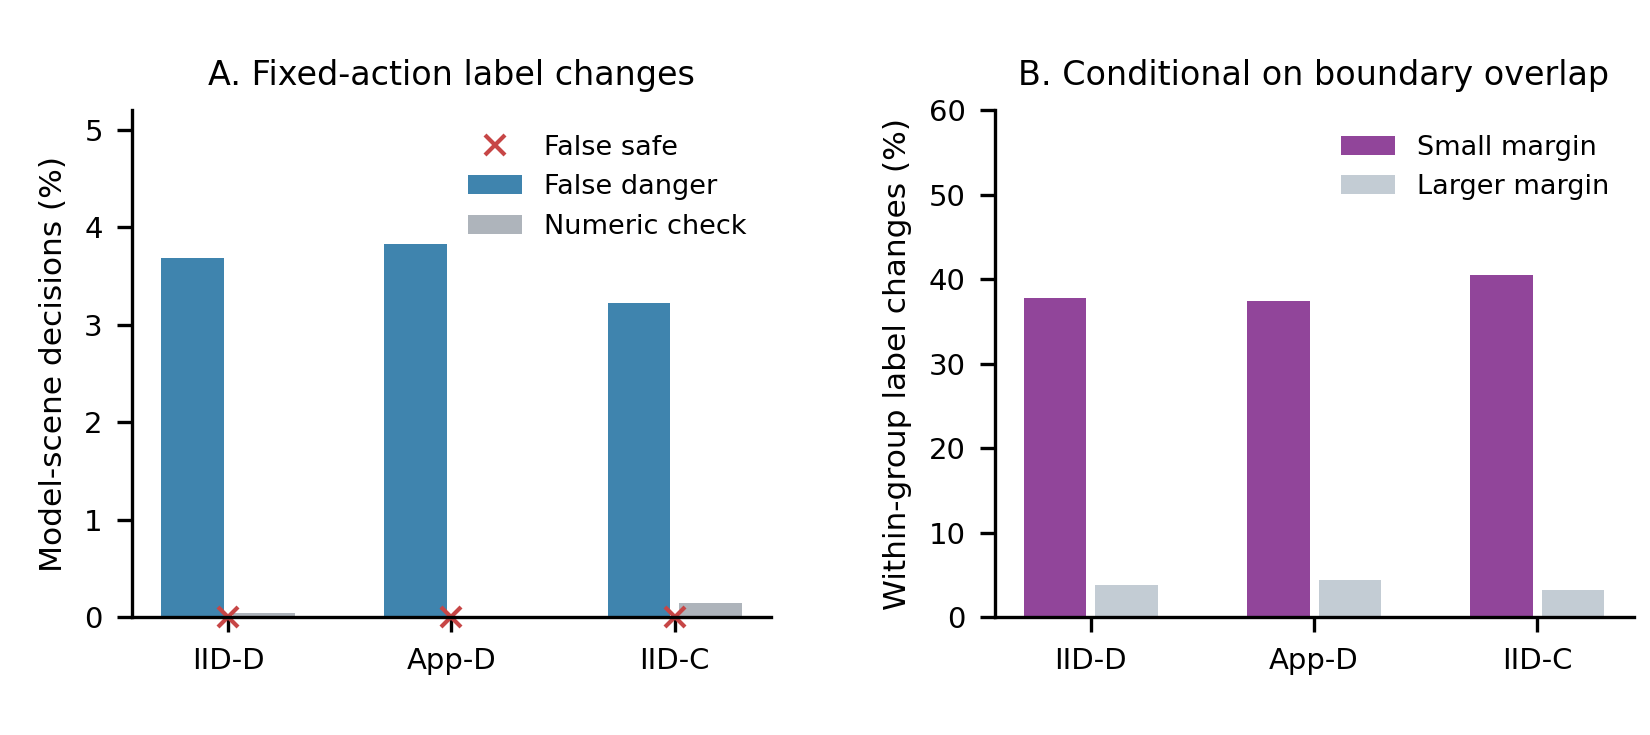
\includegraphics[width=\linewidth]{figures/oracle_confirmation.png}
\caption{Fixed-action label changes and their operating conditions. IID-D and
App-D are consumed discovery banks; IID-C is the prospective IID bank. A:
false danger means reference-safe to pooled-danger; false safe is the reverse
(no such flips observed). The numeric check holds the footprint fixed. B:
rates within overlapping-boundary groups, using the frozen .005 margin.
These are observed proportions; Table~\ref{tab:confirmation} supplies the
separate one-sided hypothesis comparisons.}
\label{fig:confirmation}
\end{figure}

Among overlapping-boundary actions, the frozen small-margin group has 40.57\%
label changes versus 3.26\% at larger margins. All 68 scenes with any flip across
models have only conservative flips, with exact conditional lower 94.1566\% for
the fixed model bank. The evidence confirms the predicted operating conditions
in the normal distribution. It does not make near-threshold sensitivity a new
general phenomenon, prove all pooling errors are positive, or establish that
every coarse decoder must lose these opportunities.
